\documentclass{article}
\usepackage{graphicx} % new way of doing eps files
\usepackage{listings} % nice code layout
\usepackage[usenames]{color} % color
\definecolor{listinggray}{gray}{0.9}
\definecolor{graphgray}{gray}{0.7}
\definecolor{ans}{rgb}{1,0,0}
\definecolor{blue}{rgb}{0,0,1}
% \Verilog{title}{label}{file}
\newcommand{\Verilog}[3]{
  \lstset{language=Verilog}
  \lstset{backgroundcolor=\color{listinggray},rulecolor=\color{blue}}
  \lstset{linewidth=\textwidth}
  \lstset{commentstyle=\textit, stringstyle=\upshape,showspaces=false}
  \lstset{frame=tb}
  \lstinputlisting[caption={#1},label={#2}]{#3}
}


\author{Steve Potter}
\title{Lab 2 - Program Counter}

\begin{document}
\maketitle

\section{Executive Summary}
The goal of this lab is to create an adder module and a mux module.  These modules will initially be used in the Fetch stage of our 64-bit ARMv8 processor.  The adder will be used to increment the Program Counter (PC).  The incremented PC will be used for sequential program execution.  The mux will be used to set the PC to either the incremented PC or to a branch address.  This selection will be based on the mux control line, which specifies whether the program should branch or continue running sequentially.

\section{Test Report}
To verify operation of these two modules, this lab requires two separate test benches.
\begin{enumerate}
	\item Adder Test Bench
	\item Mux Test Bench
\end{enumerate}

\subsection{Adder Test Bench}
The adder test bench contains:
\begin{enumerate}
	\item Inputs
	\begin{enumerate}
		\item a - the first 64-bit arithmetic operand 
		\item b - the second 64-bit arithmetic operand
	\end{enumerate}	
	\item Outputs
	\begin{enumerate}	
		\item add\_out - the 64-bit sum of the two input operands
	\end{enumerate}
\end{enumerate} 

The adder test bench sets the values of two input operands a and b and allows the adder module to produce the sum.  Correct operation is verified by comparing the Simulation Results with the Expected Results Table.  After analyzing the results, the adder works as expected.

\begin{figure}
	\begin{center}
		\caption{Expected Results of the adder test.}\label{fig:ert_addertest}
		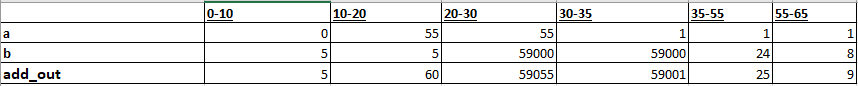
\includegraphics[width=1.0\textwidth]{../images/ert_adder_test.png}
	\end{center}
\end{figure}

\begin{figure}
	\begin{center}
		\caption{Timing diagram for the adder test.}\label{fig:addertest}
		\includegraphics[width=1.0\textwidth]{../images/adder_test.png}
	\end{center}
\end{figure}

\subsection{Mux Test Bench}
The mux test bench contains:
\begin{enumerate}
	\item Inputs
	\begin{enumerate}
		\item a - the first 64-bit mux input, which is passed to mux\_out when the control line is set to 0 
		\item b - the second 64-bit mux input, which is passed to mux\_out when the control line is set to 1
		\item control - the 1-bit control input to the mux which determines whether a or b will be passed to mux\_out
	\end{enumerate}	
	\item Outputs
	\begin{enumerate}	
		\item mux\_out - the 64-bit output of the mux
	\end{enumerate}
\end{enumerate} 

The mux test bench sets the values of a, b, and the control line and verifies that mux\_out is set to the correct value.  Correct operation is verified by comparing the Simulation Results with the Expected Results Table.  After analyzing the results, the mux works as expected.

\begin{figure}
	\begin{center}
		\caption{Expected Results of the mux test.}\label{fig:ert_muxtest}
		\includegraphics[width=1.0\textwidth]{../images/ert_mux_test.png}
	\end{center}
\end{figure}

\begin{figure}
	\begin{center}
		\caption{Timing diagram for the mux test.}\label{fig:muxtest}
		\includegraphics[width=1.0\textwidth]{../images/mux_test.png}
	\end{center}
\end{figure}

\pagebreak

\section{Code Appendix}
\Verilog{Verilog code for testing the adder.}{code:addertest}{../code/0_common/adder_test.v}
\Verilog{Verilog code for testing the mux.}{code:muxtest}{../code/0_common/mux_test.v}

\end{document} 